\documentclass{article}

\usepackage{kotex}
\usepackage{amsmath,amssymb}
\usepackage{amsthm,lipsum}
\usepackage{graphicx}% http://ctan.org/pkg/graphicx
\usepackage{listings}
\usepackage{indentfirst}
\usepackage{makecell}
\usepackage{multirow}


%package for tree
\usepackage{tikz}
\usepackage{tikz-qtree}
\usetikzlibrary{trees}

\setlength{\hoffset}{-25pt}
\addtolength{\textwidth}{50pt}
\setlength{\voffset}{-45pt}
\addtolength{\textheight}{90pt}


\begin{document}
\title{ 유전 알고리즘 프로젝트 1 보고서 }
\author{ }
\date{\today}
\maketitle


{~~}


%%%%%%%%%%%%%%%%%%%%%%%%%%%%%%%%%%%%%%%%%%%%%%%%%%%%%%%%%%%%
\section{ 사용한 GA의 구조 }

이번 과제에서는 하나의 그래프 집합을 두 개(S/S')로 나누어 그 Cut들의 합의 최대로 만드는 Maxcut 문제를 풀기 위하여 전통적인 방식의 기본 GA 연산자들을 사용하였다. GA는 기본적으로 n개의 해 집합인 Population을 무작위로 생성하고, 그것으로 알고리즘을 수행하며 해 집합을 진화시킨다.

기본적으로는 k개의 해를 Population으로부터 교체하는 Generation의 교체를 반복한다. 과정은 유전자로부터 Crossover시킬 부모를 선택하는 Selection, 선택된 두 개의 부모를 교차시키는 Crossover, 교차된 자식 유전자에 대해 특정 확률을 통해 변이시키는 Mutation. 그리고 이 과정을 통해 k개의 자손 해를 생성시키면 Population 집단으로부터 k개의 해와 교체시키는 Replacement. 이러한 하나의 Generation을 계속 반복해나가며 최적의 해를 찾아가는 방식이다.


%%%%%%%%%%%%%%%%%%%%%%%%%%%%%%%%%%%%%%%%%%%%%%%%%%%%%%%%%%%%
\subsection{ 문제 인코딩 }

이번 과제에서 주어진 Maxcut 문제는 주어진 그래프 데이터 인풋을 가지고 가장 효율적인 해의 자료구조로 녹여내는 것이 주요했다. 나의 경우, 그래프의 정보는 인풋 데이터의 형식을 그대로 따르되, 유전자의 구조는 그래프의 형질을 표현할 수 있는 것 중 가장 최소한의(S/S'를 구분하는) 구조인 binary로 표현하게 되었다.

그래프 인코딩은 기본적으로 인풋으로 주어진 그래프의 형태를 그대로 따라 (from, to, weight)를 가진 Edge의 집합으로 구성하였다. Unweighted 그래프의 경우에도 weight가 일정하게 주어져 그대로 자료구조를 사용할 수 있고, Weighted 그래프의 경우 또한 그대로 이 인코딩을 적용할 수 있기 때문이다.

해의 경우 유전자인 Chromosome을 잘 정의하는 것이 주요했다. 나의 경우, 집합 S와 S'를 나눌 수 있는 binary의 배열로 디자인하였다. 주어진 그래프에서 Vertex의 크기만큼 배열을 주고 집합 S의 속하는 경우 0을, 집합 S'에 속하는 경우 1을 주는 integer의 배열을 하나의 Chromosome 안에 넣고, 그 Choromosome의 품질을 포함하는 구조체를 자료구조로 사용하였다.


%%%%%%%%%%%%%%%%%%%%%%%%%%%%%%%%%%%%%%%%%%%%%%%%%%%%%%%%%%%%
\subsection{ GA의 세부 구조 }

GA의 기본적인 실행 구조는 주어진 제약시간 동안 여러 Generation을 거쳐서 최적의 해를 탐사하는 과정을 계속해서 거쳐나가는 것이다. 구현된 ga() 함수에서는 매 Generation, 즉 Select/Crossover/Mutation/Replace 과정을 제약시간 안에서 계속해서 반복문을 돌면서 수행해나간다. 이러한 수행과정에서 계속해서 해집단인 Population은 계속 진화해나가고, 최종적으로 제한시간 안에 끝난 유전 알고리즘은 지금까지 계산한 Population을 출력으로 내놓는다.

실험에서는 제한시간 3분이 주어졌기 때문에 그것을 확인하는 타이머를 매 Generation 마다 달아놓았고, 여기에서 3분에 도달하게 되면 GA의 수행은 종료된다.


%%%%%%%%%%%%%%%%%%%%%%%%%%%%%%%%%%%%%%%%%%%%%%%%%%%%%%%%%%%%
\subsection{ 사용한 연산자에 대한 설명 }

Selection은 처음에 두 개의 부모를 무작위로 선택하는 Random 방식을 사용하다가, Population의 각 해의 fitness를 계산하여 선택하는 Roulette Wheel 알고리즘을 사용하였다.

Crossover의 경우, 1-Point Crossover와 2-Point Crossover를 구현하여 실험해보았다. 1-Point Crossover와 2-Point Crossover 두 가지를 사용하여 실험한 이유는, 단지 1-Point Crossover와 Multipoint Crossover의 차이를 비교해보기 위함이었는데, 부모 형질을 고려하여 Cut-point를 선택하지 않는 Random Point Crossover의 경우 둘 다 큰 차이는 없었다.

Mutation은 Uniform 방식을 사용하여 Chromosome내 Random한 지점들에 대해 각각 변이시키는 방식을 선택하였다. 처음에는 Mutation Probability를 1.0\%를 주고 실험하다가 1.5\%로 바꾸어 실험을 하는 식으로 진행하였다.

Replacement는 구해진 k개의 자손 들을 Population 중 가장 품질이 나쁜 k개의 해와 교체하는 Genitor-style 방식으로 구현하고 실험하였다.


%%%%%%%%%%%%%%%%%%%%%%%%%%%%%%%%%%%%%%%%
\section{실험 및 결과}

실험 환경은 Intel(R) Core(TM) i7-7500U CPU @ 2.70GHz, Ubuntu 16.04.4 LTS의 DELL XPS 노트북으로 진행하였다. 모든 실험은 싱글 코어, 싱글 스레드를 사용하여 수행하였으며, 3분안에 종료되도록 실험하였다.

모든 실험은 각 케이스 별로 30회씩 수행하여, 그 중에 가장 우수한 결과를 채택하였다. 주어진 테스트 케이스를 사용하여 실험하였으며, 그래프 인스턴스인 Unweighted50(정점-50/간선-123), Unweighted100(정점-100/간선-495), Unweighted500(정점-500/간선-4990), Weighted500(정점-500/간선-5000), WeightedChimera297(정점-297/간선-1007)에 대해 구현한 GA을 수행시켜가면서 진행하였다. 그래프 인풋으로 주어진 정점과 간선의 갯수에 따라 인스턴스가 생성되어 프로그램이 진행되었다.

각 실험에서는 GA 내 여러 인자들을 바꾸어가며 산출된 여러 결과를 분석하며 진행되었다. 특히, Population size인 n과 Replacement size인 k, Selection과 Crossover의 전략, 그리고 변이확률인 Mutation Probability가 조정되며 실험되었다.


%%%%%%%%%%%%%%%%%%%%%%%%%%%%%%%%%%%%%%%%
\subsection{실험1 - n=100, k=20}

맨 처음에 수행해 본 가장 기본적인 실험결과이다. Population size n = 100, Replacement size k = 20를 사용하고, Selection 전략은 Random, Crossover는 1-point crossover를 사용하였다.

이번 과제에서는 Generation gap(Population size / Replacement size)을 0.2로 유지하면서, 실험을 진행하였다. 다른 여러가지 변수로 맞추어서 실험해본 결과 이게 가장 품질이 좋았기 때문이다. 처음에는 단순하게 Population size가 크면, 초기에 탐색하는 공간에서 넓은 범위를 가질 확률이 높다고 생각해서 n을 크게 주고 실험해보았다. 품질은 생가보다 나쁘지 않았다. 각 인스턴스별로 최적해에 못 도달하긴 했지만 그래도 근사한 값이 나왔다.



%%%%%%%%exp table%%%%%%%%%
 \begin{table}[h]
 \begin{center}
\caption{실험1 결과}
\begin{tabular}{cccc}
\hline\hline
케이스 & 평균 결과 & 최고 결과 & 표준편차\\
\hline\hline
$Unweighted 50$ & 95.8 & 96 & 0.7\\
\hline
$Unweighted 100$ & 348.3 & 349 & 2.0\\
\hline
$Unweighted 500$ & 3088.2 & 3098 & 15.3\\
\hline
$Weighted 500$ & 4248.2 & 4267 & 33.8\\
\hline
$Weighted Chimera 297$ & 8070.6 & 8456 & 853.3\\
\hline
\end{tabular}
\end{center}
\end{table}
%%%%%%%%exp table%%%%%%%%%
%%%%%%%%%%%%%%%%%%%%%%%%%%%%%%%%%%%%%%%%


%%%%%%%%%%%%%%%%%%%%%%%%%%%%%%%%%%%%%%%%
\subsection{실험2 - n=50, k=10}

이번에는 n과 k를 각각 실험1의 반으로 낮추어, Population size n = 50, Replacement size k = 10를 사용하고, Selection과 Crossover는 그대로 놓고 실험하였다.

이 실험결과도 실험1과 비슷한 추이를 보였다. Population size는 유전자 해의 품질에 크게 영향을 미치지는 않는 것 같다. 하지만, 크기를 조금 낮추었을 때, 보이는 Generation evoltion 횟수의 증가가 실험1과 비교되어 다만 이것을 좀 더 잘 확인해보고자 n을 조금 더 낮추어 보아야겠다는 생각을 하였다.



%%%%%%%%exp table%%%%%%%%%
 \begin{table}[h]
 \begin{center}
\caption{실험2 결과}
\begin{tabular}{cccc}
\hline\hline
케이스 & 평균 결과 & 최고 결과 & 표준편차\\
\hline\hline
$Unweighted 50$ & 98.6 & 99 & 0.7\\
\hline
$Unweighted 100$ & 347.3 & 348 & 1.5\\
\hline
$Unweighted 500$ & 3096.9 & 3107 & 11.9\\
\hline
$Weighted 500$ & 4214 & 4225 & 21.6\\
\hline
$Weighted Chimera 297$ & 8433.2 & 8864 & 855.8\\
\hline
\end{tabular}
\end{center}
\end{table}
%%%%%%%%exp table%%%%%%%%%
%%%%%%%%%%%%%%%%%%%%%%%%%%%%%%%%%%%%%%%%


%%%%%%%%%%%%%%%%%%%%%%%%%%%%%%%%%%%%%%%%
\subsection{실험3 - n=20, k=4}

실험3에서는 n을 더 낮추어 20으로, Replacement size k = 4를 사용하고, Selection과 Crossover는 그대로 두고 실험하였다.

이 실험은 앞선 실험 1,2의 진행에 맞추어 Population size를 계속해서 낮춘 것이었다. 실험 1,2와 비교해보았을 때 해의 품질이 크게 차이나진 않았다. 그러나 실험 3 또한 실험 2와 마찬가지로 n의 크기를 낮추면서 GA 연산자들의 수행 횟수라 볼 수 있는 Generation의 Evolution 수가 늘었기 때문에, 이 정도에서 n과 k를 고정하고 다른 변수를 바꾸어가며 다른 전략을 바꾸어 실험을 해보기로 하였다.


%%%%%%%%exp table%%%%%%%%%
 \begin{table}[h]
 \begin{center}
\caption{실험3 결과}
\begin{tabular}{cccc}
\hline\hline
케이스 & 평균 결과 & 최고 결과 & 표준편차\\
\hline\hline
$Unweighted 50$ & 96 & 96 & 0.2\\
\hline
$Unweighted 100$ & 352.4 & 354 & 2.1\\
\hline
$Unweighted 500$ & 3090.5 & 3112 & 18.2\\
\hline
$Weighted 500$ & 4258.1 & 4307 & 45.1\\
\hline
$Weighted Chimera 297$ & 8232.4 & 8501 & 703.3\\
\hline
\end{tabular}
\end{center}
\end{table}
%%%%%%%%exp table%%%%%%%%%
%%%%%%%%%%%%%%%%%%%%%%%%%%%%%%%%%%%%%%%%

%%%%%%%%%%%%%%%%%%%%%%%%%%%%%%%%%%%%%%%%
\subsection{실험4 - Mutation Probability의 조정}

Population size n = 20, Replacement size k = 4를 사용하고, Selection 전략은 Random, Crossover는 1-point crossover를 사용하였다. 기본적인 조건은 거의 비슷하지만, 이번에는 Mutation 연산시 영향을 미치는 Mutation probability를 1.5\%에서 1\%로 낮추어보았다.

실험한 결과, 이 것도 역시나 큰 차이를 얻을 수는 없었다. Mutation probability를 큰 차이로 바꾸어 다시 실험해보았으나, 그 결과는 이것보다도 좋지못해, 그냥 가장 합리적인 1.5\%에서 더이상 건드리지 않기로 하였다.\linebreak\linebreak\linebreak


%%%%%%%%exp table%%%%%%%%%
 \begin{table}[h]
 \begin{center}
\caption{실험4 결과}
\begin{tabular}{cccc}
\hline\hline
케이스 & 평균 결과 & 최고 결과 & 표준편차\\
\hline\hline
$Unweighted 50$ & 94.9 & 95 & 0.2\\
\hline
$Unweighted 100$ & 349.9 & 350 & 0.2\\
\hline
$Unweighted 500$ & 3185.1 & 3193 & 12.8\\
\hline
$Weighted 500$ & 4360.4 & 4371 & 25.4\\
\hline
$Weighted Chimera 297$ & 8199.4 & 8476 & 671\\
\hline
\end{tabular}
\end{center}
\end{table}
%%%%%%%%exp table%%%%%%%%%
%%%%%%%%%%%%%%%%%%%%%%%%%%%%%%%%%%%%%%%%

%%%%%%%%%%%%%%%%%%%%%%%%%%%%%%%%%%%%%%%%
\subsection{실험5 - Selection 전략의 변경}

위 n, k, Mutation probability 같은 변수들을 여럿 바꾸어가면서 실험해보았다. 이번에는 GA 연산자의 전략, 즉 알고리즘을 수정하는 방향으로 실험해보았는데, 기존에 Selection 방식에서 무작위로 두 부모를 선택하는 방식에서 fitness를 계산해 각각의 선택에 반영하는 방식으로 바꾸어 실험해보았다.

Selection 전략을 바꾼 결과는 생각보다 효과적이었다. 아무래도, 두 부모를 선택할 때 우수한 형질에 대해 좀 더 우선순위를 주도록 구현해서 그런지, 우수해에 가까운 쪽으로 수렴하는 양상을 보였다.


%%%%%%%%exp table%%%%%%%%%
 \begin{table}[h]
 \begin{center}
\caption{실험5 결과}
\begin{tabular}{cccc}
\hline\hline
케이스 & 평균 결과 & 최고 결과 & 표준편차\\
\hline\hline
$Unweighted 50$ & 98.6 & 99 & 1.23\\
\hline
$Unweighted 100$ & 349.9 & 351 & 2.6\\
\hline
$Unweighted 500$ & 3105.6 & 3117 & 20.2\\
\hline
$Weighted 500$ & 4366.75 & 4396 & 30.8\\
\hline
$Weighted Chimera 297$ & 8416 & 8864 & 1007.3\\
\hline
\end{tabular}
\end{center}
\end{table}
%%%%%%%%exp table%%%%%%%%%
%%%%%%%%%%%%%%%%%%%%%%%%%%%%%%%%%%%%%%%%

%%%%%%%%%%%%%%%%%%%%%%%%%%%%%%%%%%%%%%%%
\subsection{실험6 - Crossover 전략의 변경}

위 실험 5에 이어서, 이번에는 1-Point Crossover를 Multipoint Crossover로 바꾸어 실험해보기로 하였다. 처음에는 무작위 p개의 Point들을 잡고 Crossover시키는 방식으로 구현하려 했으나, 오버헤드가 크고 별로 효과적이지 못한 결과를 보여, 그냥 2-Point Crossover를 구현하여 1-Point Crossover와의 차이를 비교하려 하였다.

결과는 생각보다 좋지 않았다. 오히려 품질이 떨어진 부분도 있었고, 전반적으로 결과는 비슷하게 나왔으나 향상되지는 못하였다. 1-Point이던 2-Point이던 교차시키는 부모의 형질을 고려하는 것이 아닌 무작위의 Cut 지점을 잡는 것이 무의미해서 그런 것 같았다.

%%%%%%%%exp table%%%%%%%%%
 \begin{table}[h]
 \begin{center}
\caption{실험6 결과}
\begin{tabular}{cccc}
\hline\hline
케이스 & 평균 결과 & 최고 결과 & 표준편차\\
\hline\hline
$Unweighted 50$ & 95.8 & 96 & 0.6\\
\hline
$Unweighted 100$ & 355.7 & 356 & 1.1\\
\hline
$Unweighted 500$ & 3116.2 & 3125 & 15.3\\
\hline
$Weighted 500$ & 4437.2 & 4458 & 36\\
\hline
$Weighted Chimera 297$ & 8369.7 & 8864 & 1089.1\\
\hline
\end{tabular}
\end{center}
\end{table}
%%%%%%%%exp table%%%%%%%%%
%%%%%%%%%%%%%%%%%%%%%%%%%%%%%%%%%%%%%%%%


%%%%%%%%%%%%%%%%%%%%%%%%%%%%%%%%%%%%%%%%%%%%%%%%%%%%%%%%%%%%
\section{ 결과 분석 }

여러 번의 실험결과 Population size와 Replacement size는 특별히 작거나 크지 않다면 품질에 크게 영향을 주지 않는다는 것을 확인할 수 있었다. 그 대신, GA 연산자 내에 전략이라던가, 해의 공간탐색에 있어 유리한 시도를 하는 편이 좀 더 품질에 대한 영향을 주는 요소가 더 많았다. 그리고 또한, Generation의 진화 횟수를 늘릴 수록 좋은 해의 양상이 보인 다는 것을 판단할 수 있었다. 하지만 이러한 모든 수행결과는 전통적인 GA를 돌렸을 때의 한계점을 나타내고 있었다. 사실 변수별로 어느 정도 차이는 있었지만, 바꾸어도 전통적 GA에서 가지는 한계는 극복하기 힘들었던 것 같다.

마지막으로 가장 최종적으로 우수한 해를 나타낸 n=20, k=4, MutationProb=0.015, Roulette Wheel Selection, One-point Crossover를 통해 실험한 결과에서 수행된 Population의 진화 양상을 분석하였다. 실험은 Weighted Chimera 297 그래프 데이터에 대해서 평균 해의 품질과 해의 최고 품질의 수렴하는 양상을 분석한 것이다.

\begin{figure}[h]
  \centering
  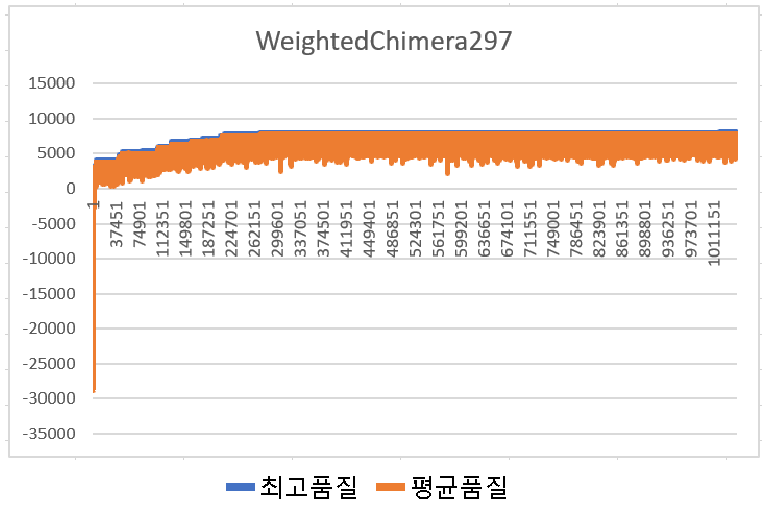
\includegraphics[width=1.0\textwidth]{chimera_chart.pdf}
  \label{figure1}
\end{figure}


위 그래프와 같이 초기에 Population이 생성된 후, 빠른 속도로 최적해에 수렴해가다가, 일정 수준을 지난 이후로는 그 양상이 완만해지는 것을 확인할 수 있었다. 총 100만여번의 Generation 진화의 수행과정 중, 20만번에 이르면 최적해에 많이 수렴하고, 그 이후의 진화과정은 완만한 형태를 이루는 것을 관찰할 수 있었다.


%%%%%%%%%%%%%%%%%%%%%%%%%%%%%%%%%%%%%%%%%%%%%%%%%%%%%%%%%%%%
\section{ 논의 }

사실 전통적인 GA의 방식으로 품질변화가 눈에 띄게 보이는 품질 향상을 만들어내기는 어려웠다. 여러가지 시행착오를 겪으며 그나마 가장 최적해에 가까운 값을 찾았다고는 했으나, 그래도 많이 부족한 감이 없지는 않았다. 실험 관찰 결과 재미있었던 것은 초기 Initial population 생성된 해의 품질이 결과적으로 나타난 해에 영향을 많이 미친다는 것이었다. 여러가지 변수의 변화도 중요하지만 초기 Population의 품질이 이후 진화하는 해 집합의 품질에 큰 영향을 미치게 되었다.

이러한 분석 결과, 초기에 Population을 문제에 대한 정보를 이용하여 잘 줄 수 있으면 좀 더 좋은 해를 얻을 수 있을 것 같다는 결론을 얻을 수 있었다. 이번 과제에서는 전통적인 GA 방식 이외에 다른 최적화와 지역 최적화를 사용할 수 없어서 만들어내는 품질에 한계가 있었던 것 같다. 이후의 과제에서 여러가지 방법을 사용하면 더 좋은 품질을 낼 수 있을 것 같다.

% if exists, reference
%\begin{thebibliography}{3}
%\bibitem{p200}
%Dawson Engler and Ken Ashcraft,
%`` RacerX: Effective, Static Detection of Race Conditions and Deadlocks'',
%\emph{SOSP’03}, 
%October 19–22, 2003
%\end{thebibliography}

%\appendix
%\section{Appendix Title}

%This is the text of the appendix, if you need one.

\end{document}

